\documentclass[9pt]{article}

\usepackage{amssymb}
\usepackage{amsmath}
\usepackage{amsfonts}
\usepackage{comment}
\usepackage{fancyhdr}
\usepackage{mathrsfs}
\usepackage{enumitem}
\usepackage{url}
\expandafter\def\expandafter\UrlBreaks\expandafter{\UrlBreaks%  save the current one
  \do\a\do\b\do\c\do\d\do\e\do\f\do\g\do\h\do\i\do\j%
  \do\k\do\l\do\m\do\n\do\o\do\p\do\q\do\r\do\s\do\t%
  \do\u\do\v\do\w\do\x\do\y\do\z\do\A\do\B\do\C\do\D%
  \do\E\do\F\do\G\do\H\do\I\do\J\do\K\do\L\do\M\do\N%
  \do\O\do\P\do\Q\do\R\do\S\do\T\do\U\do\V\do\W\do\X%
  \do\Y\do\Z}


\usepackage{tikz}

\voffset = -50pt
%\textheight = 700pt
\addtolength{\textwidth}{60pt}
\addtolength{\evensidemargin}{-30pt}
\addtolength{\oddsidemargin}{-30pt}
%\setlength{\headheight}{44pt}

\pagestyle{fancy}
\fancyhf{} % clear all fields
\fancyhead[R]{%
  \scshape
  \begin{tabular}[t]{@{}r@{}}
  CECS 424, Summer 2015\\Section 1 (11171)\\
  HW \#1, DUE: 2015, July 13
  \end{tabular}}
\fancyhead[L]{%
  \scshape
  \begin{tabular}[t]{@{}r@{}}
  JOSEPH OKONOBOH\\Computer Science\\Cal State Long Beach
  \end{tabular}}
\fancyfoot[C]{\thepage}

\newcommand{\qed}{\hfill \ensuremath{\Box}}


\newcommand*\circled[1]{\tikz[baseline=(char.base)]{
            \node[shape=circle,draw,inner sep=2pt] (char) {#1};}}

\newcommand{\Z}{\mathbb{Z}}
\newcommand{\I}{\mathbb{I}}
\newcommand{\M}{\mathbb{M}}
\newcommand{\Q}{\mathbb{Q}}
\newcommand{\R}{\mathbb{R}}
\newcommand{\C}{\mathbb{C}}
\newcommand{\D}{\displaystyle}
%\setcounter{section}{-1}

\begin{document}
\noindent Complete these problems on a separate sheet of paper. Due July 14 at
the beginning of lecture.
\begin{enumerate}
%%%%%%%%%%%%%%%%%%%%%%%%%%%%%%%%%%%%%%%01%%%%%%%%%%%%%%%%%%%%%%%%%%%%%%%%%%%%%%%
   \item Reading:

         \begin{enumerate}
            \item Chapter 1 intro
            \item \textit{Skim} Chapter 1.1, 1.2, 1.3
            \item Chapter 1.4, 1.6
            \item Chapter 2 intro
            \item Chapter 2.1
            \item Chapter 3 intro
            \item Chapter 3.1, 3.2
         \end{enumerate}
%%%%%%%%%%%%%%%%%%%%%%%%%%%%%%%%%%%%%%%02%%%%%%%%%%%%%%%%%%%%%%%%%%%%%%%%%%%%%%%
   \item \textit{Structured programming} is sometimes distinguished from
         \textit{prodecural programming} by the removal of \verb|jump/goto|
         operations found in procedural languages. The \verb|goto| statement has
         received decades of ire from academic and professional computer
         scientists since Edsger Dijkstra's 1968 essay ``Go To Considered
         Harmful." With few exceptions (C++), almost all ``modern" progamming
         languages forbid the use of \verb|goto-|like statements, with some
         languages (Java) going so far as to make \verb|goto| a reserved keyword
         that throws a compile-time error for anyone who attempts to use it.
         However, there remain convincing arguments in favor of using
         \verb|goto| in specific disciplined ways, and languages without the
         \verb|goto| statement must make other facilities available as 
         alternatives. \\

         In a one- or two-paragraph response, summarize the case for removing
         \verb|goto| statements from structured programming languages. Include
         in your response at least one programming problem whose solution is
         easier using \verb|goto| statements but does not exhibit many of the
         arguments against \verb|goto|. Do you feel the case against \verb|goto|
         is strong enough to ban its inclusion in modern languages?
         
      \textbf{Answer.} 
      
      \begin{itemize}
         \item \textbf{Debug.} The \verb|goto| construct may contribute to
               difficulty in debugging a program because the program's natural
               control flow may be interrupted.
         \item \textbf{State.} A \verb|goto| instruction may cause the program
               to jump to portions of the code where variables are not in a
               consistent or expected state.
      \end{itemize}
      
      One situation in which the \verb|goto| statement is more natural than
      other substitutes is in multiple nested loops. The programmer can easily
      use the \verb|goto| statement to break out of these loops, as opposed to
      using more involved awkard constructs. For example, to achieve this in
      Java, one would have to use a label, which is, incidentally, similar to
      using a \verb|goto| statement. I believe most programmers do not use
      \verb|goto| not because they truly understand the ``damage" it can cause,
      but because they were simply told that it was bad. There is a plethora of
      badly written programs that do not use \verb|goto|; indeed, the
      \verb|goto| statement does not turn a good programmer into a bad one; it
      simply gives the bad one more options to hang himself with. Thus if a
      programmer uses this statement in a respectful and natural way, he can
      more easily solve particular problems. Unfortunately, the definitions of
      ``respectful" and ``meaningful" in this context are up to the discretion
      of the programmer. Nevertheless, I do not agree that such a powerful
      programming construct should be taken away from a programmer, because a
      programmer should be able to shoot himself in the foot if he sees fit.      
%%%%%%%%%%%%%%%%%%%%%%%%%%%%%%%%%%%%%%%03%%%%%%%%%%%%%%%%%%%%%%%%%%%%%%%%%%%%%%%
   \item Read about the ``goto fail" bug in Apple's iOS/OSX SSL connection
         libraries from 2014. In a one-paragraph response, summarize the error's
         cause, and decide whether you believe the use of \verb|goto| in the
         flawed code was a primary cause of the error. If you blame \verb|goto|,
         demonstrate how to reorganize the code without \verb|goto| to eliminate
         the error; if \verb|goto| is not to blame, describe other programming
         or cultural practices that could have prevented the error being
         published.

      \textbf{Answer.} The snippet of code below was part of the original faulty
      code. The modified one can be found at \url{http://opensource.apple.com/source/Security/Security-55471/libsecurity_ssl/lib/sslKeyExchange.c}
\begin{verbatim}
1.    hashOut.data = hashes + SSL_MD5_DIGEST_LEN;
2.    hashOut.length = SSL_SHA1_DIGEST_LEN;
3.    if ((err = SSLFreeBuffer(&hashCtx)) != 0)
4.       goto fail;
5.    if ((err = ReadyHash(&SSLHashSHA1, &hashCtx)) != 0)
6.       goto fail;
7.    if ((err = SSLHashSHA1.update(&hashCtx, &clientRandom)) != 0)
8.       goto fail;
9.    if ((err = SSLHashSHA1.update(&hashCtx, &serverRandom)) != 0)
10.      goto fail;
11.   if ((err = SSLHashSHA1.update(&hashCtx, &signedParams)) != 0)
12.      goto fail;
13.      goto fail;
14.   if ((err = SSLHashSHA1.final(&hashCtx, &hashOut)) != 0)
15.      goto fail;
\end{verbatim}

As we can see, line 13 is problematic because if \verb|err == 0| is true in
line 11 (that is, no error occurred  from calling
\verb|SSLHashSHA1.update(&hashCtx, &signedParams)|), then line 12 will not
execute. However, in this case, line 13 will unconditionally execute, thus
unwittingly trigerring some fail procedure. \\

I believe that the primary cause of this error was less about the use of \verb|goto|
than the carelessness of the programmer. Personally I tend to use braces around
all my \verb|if| statements, whether or not they have a single statement of
code. If the coding convention had included using braces around every \verb|if|
statements, then perhaps, the error might have been patent from the onset.

%%%%%%%%%%%%%%%%%%%%%%%%%%%%%%%%%%%%%%%04%%%%%%%%%%%%%%%%%%%%%%%%%%%%%%%%%%%%%%%
   \item (Exercise 1.1 from \textit{Programming Language Pragmatics}) Using the
         C programming language, give an example of each of the following:

         \begin{enumerate}
            \item A lexical error, detected by the scanner/lexer.
            \item A syntax error, detected by the parser.
            \item A static semantic error, detected by semantic analysis.
            \item A dynamic semantic error, detected by code generated by the
                  compiler.
         \end{enumerate}

      \textbf{Solution.}

      \begin{enumerate}
         \item \begin{verbatim}
1. // There is a lexical error on line 4.
2.
3. int main() {
4.    int 123x = 90;
5.    return 0;
6. }
         \end{verbatim}
         \item \begin{verbatim}
1. // There is a syntax error on line 5.
2
3. int main() {
4.    int x = 90;
5.    = int;
6.    return 0;
7. }
         \end{verbatim}
         \item \begin{verbatim}
1. // There is a static semantic error on line 4.
2.
3. int main() {
4.    int x = "String";
5.    return 0;
6. }
         \end{verbatim}
         \item \begin{verbatim}
1. // There is a dynamic semantic error on line 6.
2.
3. int main() {
4.    int y = 0;
5.    int* z = (int*) y;
6.    *z = 89;
7.    return 0;
8. }
         \end{verbatim}
      \end{enumerate}
%%%%%%%%%%%%%%%%%%%%%%%%%%%%%%%%%%%%%%%05%%%%%%%%%%%%%%%%%%%%%%%%%%%%%%%%%%%%%%%
   \item Use the following grammar to draw a parse tree for the expression
         \verb|(3+4)*5:|

         \begin{itemize}
            \item \textit{expr} $\rightarrow$ \textit{term $|$ expr add\_op term}
            \item \textit{term} $\rightarrow$ \textit{factor $|$ term mult\_op 
                  factor}
            \item \textit{factor} $\rightarrow$ \texttt{id $|$  number $|$ - }
                  \textit{factor} $|$ \verb|(|$expr$\verb|)|
            \item \textit{add\_op} $\rightarrow$ \verb|+| $|$ \verb|-|
            \item \textit{mult\_op} $\rightarrow$ \verb|*| $|$ \verb|/|
         \end{itemize}
         
      \textbf{Solution.}
      
      \begin{center}
         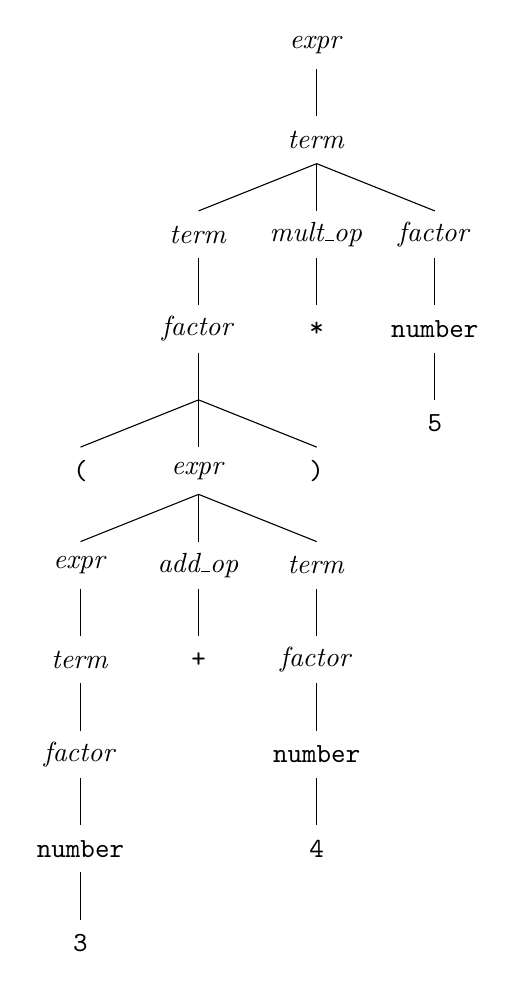
\begin{tikzpicture}[scale=3.0]
            %\draw[step=.5cm,gray,very thin] (-2.0,-2.0) grid (2.0, 2.0);
            \draw (0.0,2.0) node {\textit{expr}};
            
            \draw (0.0,1.9) -- (0.0, 1.7);
            
            \draw (0.0,1.6) node {\textit{term}};
            
            \draw (0.0,1.5) -- (-0.5, 1.3);            
            \draw (0.0,1.5) -- (0.0, 1.3);
            \draw (0.0,1.5) -- (0.5, 1.3);
            
            \draw (-0.5,1.2) node {\textit{term}};
            \draw (0.0,1.2) node {\textit{mult\_op}};
            \draw (0.5,1.2) node {\textit{factor}};
            
            \draw (-0.5,1.1) -- (-0.5, 0.9);
            \draw (0.0,1.1) -- (0.0, 0.9);
            \draw (0.5,1.1) -- (0.5, 0.9);
            
            \draw (-0.5,0.8) node {\textit{factor}};
            \draw (0.0,0.8) node {\verb|*|};
            \draw (0.5,0.8) node {\verb|number|};
            
            \draw (-0.5,0.7) -- (-0.5, 0.5);
            \draw (0.5,0.7) -- (0.5, 0.5);
            
            \draw (-0.5,0.5) -- (-1.0, 0.3);
            \draw (-0.5,0.5) -- (-0.5, 0.3);
            \draw (-0.5,0.5) -- (0.0, 0.3);
            \draw (0.5,0.4) node {\verb|5|};
            
            \draw (-1.0,0.2) node {\verb|(|};
            \draw (-0.5,0.2) node {\textit{expr}};
            \draw (0.0,0.2) node {\verb|)|};
            
            \draw (-0.5,0.1) -- (-1.0, -0.1);
            \draw (-0.5,0.1) -- (-0.5, -0.1);
            \draw (-0.5,0.1) -- (0.0, -0.1);
            
            \draw (-1.0, -0.2) node {\textit{expr}};
            \draw (-0.5, -0.2) node {\textit{add\_op}};
            \draw (0.0, -0.2) node {\textit{term}};
            
            \draw (-1.0, -0.3) -- (-1.0, -0.5);
            \draw (-0.5, -0.3) -- (-0.5, -0.5);
            \draw (0.0, -0.3) -- (0.0, -0.5);
            
            \draw (-1.0, -0.6) node {\textit{term}};
            \draw (-0.5, -0.6) node {\verb|+|};
            \draw (0.0, -0.6) node {\textit{factor}};
            
            \draw (-1.0, -0.7) -- (-1.0, -0.9);
            \draw (0.0, -0.7) -- (0.0, -0.9);
            
            \draw (-1.0, -1.0) node {\textit{factor}};
            \draw (0.0, -1.0) node {\verb|number|};
            
            \draw (-1.0, -1.1) -- (-1.0, -1.3);
            \draw (0.0, -1.1) -- (0.0, -1.3);
            
            \draw (-1.0, -1.4) node {\verb|number|};
            \draw (0.0, -1.4) node {\verb|4|};
            
            \draw (-1.0, -1.5) -- (-1.0, -1.7);
            \draw (-1.0, -1.8) node {\verb|3|};
         \end{tikzpicture}
      \end{center}
%%%%%%%%%%%%%%%%%%%%%%%%%%%%%%%%%%%%%%%06%%%%%%%%%%%%%%%%%%%%%%%%%%%%%%%%%%%%%%%
   \item Explain in your own words why a language that only supports
         \textit{static allocation} of values cannot support recursive
         functions.
         
      \textbf{Answer.} For recursive functions to execute correctly, then each
      invocation of a particular function call must have its own unshared
      local variables, if any. However, if the language only supports static
      allocation, each successive function invocation in a recursive call will
      overwrite the data of the previous function call, and this may lead to
      logical errors in the program.
%%%%%%%%%%%%%%%%%%%%%%%%%%%%%%%%%%%%%%%07%%%%%%%%%%%%%%%%%%%%%%%%%%%%%%%%%%%%%%%
   \item In the following C program, identify one value/object that is allocated
         statically, one that is allocated on the stack, and one that is
         allocated on the heap. Be specific.

         \begin{verbatim}
int global;
int main() {
   scanf("%d", &global); // read an integer form standard in
   int *arr = (int*)malloc(global * sizeof(int)); // allocate an array of the
                                                  // desired size.

   for (int i = 0; i < global; i++) {
      scanf("%d", &arr[i]) // scan in one int for each array location
   }
   return 0;
}
         \end{verbatim}

      \textbf{Answer.}

      $$
         \begin{tabular}{@{}|c|c|@{}} \hline
            Allocation Type & Object \\ \hline
            Static & \verb|global| \\ \hline
            Stack  & \verb|i| \\ \hline
            Heap   & \verb|*arr| \\ \hline
         \end{tabular}
      $$
%%%%%%%%%%%%%%%%%%%%%%%%%%%%%%%%%%%%%%%08%%%%%%%%%%%%%%%%%%%%%%%%%%%%%%%%%%%%%%%
   \item Describe what the followng \textit{format specifiers} will print when
         used with the C function \verb|printf|, assuming appropriate values are
         passed as arguments:
         \begin{enumerate}
            \item \verb|%d|
            \item \verb|%s|
            \item \verb|%f|
            \item \verb|%e|
            \item \verb|%%|
         \end{enumerate}

      \textbf{Answer.}

      \begin{enumerate}
         \item The format specifier \verb|%d| will print a signed decimal
               integer.
         \item The format specifier \verb|%s| will print a null terminated
               string.
         \item The format specifier \verb|%f| will print a floating point
               number.
         \item The format specifier \verb|%e| will print a number in scientific
               notation.
         \item The format specifier \verb|%%| will print the literal character
               `\verb|%|'.
      \end{enumerate}
\end{enumerate}
\end{document}
